\section{Introduction}
\label{sec:intro}

Pretrained forecasting models such as TimesFM \citep{das2024timesfm}, the Chronos family
\citep{ansari2024chronos,ansari2025chronos2}, Sundial \citep{liu2025sundial}, Timer \citep{liu2024timer} and Time-MoE
\citep{shi2025timemoe} are released as open checkpoints and used zero-shot. They are built very differently. TimesFM
reads 32-step patches with a decoder; Chronos-T5 quantizes every time step into a vocabulary and runs an
encoder--decoder; Chronos-2 is an encoder with cross-series attention; Sundial samples its forecast from a flow-matching
head; Timer reads 96-step tokens. Benchmarks rank them by accuracy but do not tell us what they represent. In
vision and language, networks trained on similar data are argued to converge on similar representations
\citep{li2016convergent,huh2024platonic}. It is not known whether
forecasting models with such different inductive biases do the same, or whether any shared structure affects the
forecast.

We study this question for seven TSFMs. Three properties of forecasting models make the standard interpretability
toolkit \citep{kornblith2019cka,meng2022rome,bricken2023monosemanticity} hard to apply directly, and in each case the
failure is a plausible but wrong result rather than an error. Tokens cover between 1 and 96 time steps depending on the
model, so activations must be placed on a common time axis before they can be compared. Real series carry no labels for
trend, seasonality or noise, so a probe that appears to find seasonality cannot be checked on them. And removing a single
internal feature typically moves a forecast by about a tenth of the context's standard deviation, small enough that a
poorly chosen null or a precision mismatch can produce spurious effects. We therefore measure each model's token-to-time
map, use generated benchmarks with exact ground truth, validate the causal instruments on a forecaster with planted
concepts and decoys, and test registered claims once on sealed held-out splits of two corpora
(Section~\ref{sec:methods}).

Our results fall into three groups. The first concerns what the models share (Section~\ref{sec:shared}). All 21 model
pairs have representational geometry above chance, confirmed on a fresh sealed split, and concepts transfer across
architectures at the level of inputs. For a concept found in one model, features in the other models select the same
series, and all registered transfer claims confirm on both corpora and on 800 raw real-world windows that were never used
during development.

The second concerns how the models differ (Section~\ref{sec:mechanisms}). Causal features act mostly on the level and
seasonality of the forecast, and features that raise level, lower level or damp seasonality occur in every model.
Finer-grained concepts, however, are organized by model, and none spans more than three of the seven. The same function
can be implemented by one attention head in TimesFM and by five interacting heads in Chronos-T5-Base. Forecast-relevant
information also appears to be distributed, since single features stand out only modestly against random directions
drawn from the activation distribution. We detect the same causal effect on the same series only between Chronos-2 and
Chronos-Bolt.

The third concerns methodology (Section~\ref{sec:shortcuts}). Averaging the tokens in a time window, the usual way of
comparing models with different tokenizers, understates TimesFM's similarity to fine-token models by 0.30--0.43 CKA.
Of the most frequently and strongly active dictionary features, 83.5\% have no held-out causal effect. Attention to
seasonal lags is uncorrelated with which heads carry seasonality, and a random-direction null that ignores a feature's
per-token activation profile inflates the number of causal features 2.7-fold.

In addition, the depths at which TimesFM and Chronos-2 respond to input corruptions agree in a way that replicates for
most corruptions, and internal features improve failure prediction only for the two least accurate models
(Section~\ref{sec:depth}). Each result is recorded, with its evidence class, exact numbers and a reproduction command, in
a public findings ledger (\repo{FINDINGS.md}); identifiers such as \fid{SH-18} refer to its entries. The analysis
software and benchmark generator are open source (Appendix~\ref{app:system}).

\begin{figure}[!tb]
\centering
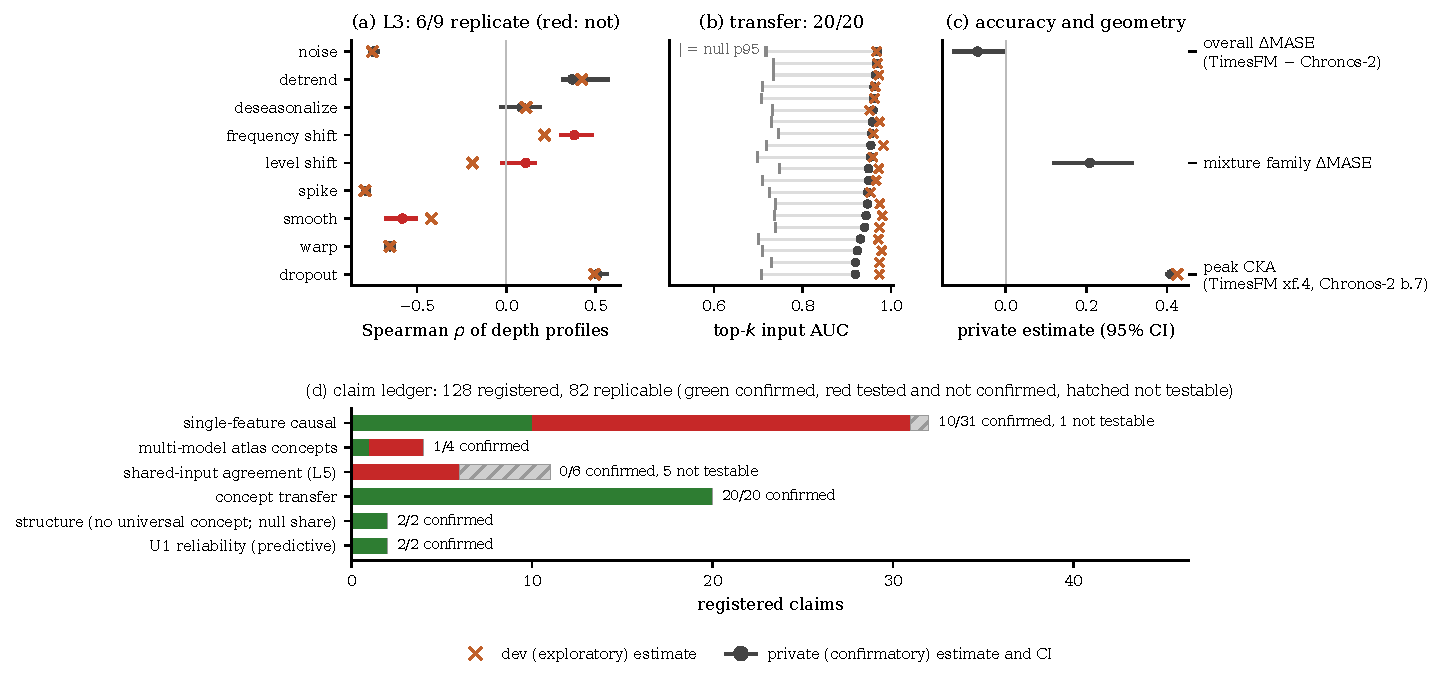
\includegraphics[width=\textwidth]{heldout.pdf}
\caption{Claims re-tested once on the sealed v2 private split (971 series; panel a uses 800 of them). (a) Per-corruption
depth-profile agreement, TimesFM vs.\ Chronos-2 (red: the dev value is not inside the private interval). (b) The 20
concept-transfer claims with private null 95th percentiles. (c) Accuracy and peak CKA; crosses are
dev values, dots and bars private values with 95\% series-bootstrap intervals. (d) Registered concept claims by
type. Source:
\texttt{confirm/confirmation.json}.}
\label{fig:heldout}
\end{figure}
